\section{Programming}
\label{sec:programming}

Now that the constraints have been added, we can generate the .bit file that will be
programmed to the FPGA.
The steps that are required are to run Synthesis, Implementation, and then Generate Bitstream.
However, as a shortcut, you can click on Generate Bitstream and it will automatically run the
other steps if they need to be run.

\begin{center}
    \begin{tikzpicture}[arrow/.style={-latex, line width=10pt, darkred!70}]
    \node[anchor=south west,inner sep=0] (image) at (0,0)
    {
        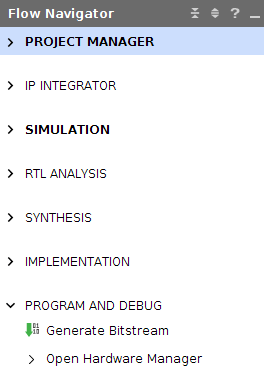
\includegraphics{project_flow_generate_bitstream}
    };
    \begin{scope}[x={(image.south east)},y={(image.north west)}]
        \node (start) at (0.95,0.12) {};
        \node [left of=start, xshift=-1.2cm] (end) {};
        \draw [arrow] (start) -- node [midway, black] {} (end);
    \end{scope}
    \end{tikzpicture}
\end{center}
\begin{center}
    \begin{tikzpicture}[arrow/.style={-latex, line width=10pt, darkred!70}]
    \node[anchor=south west,inner sep=0] (image) at (0,0)
    {
        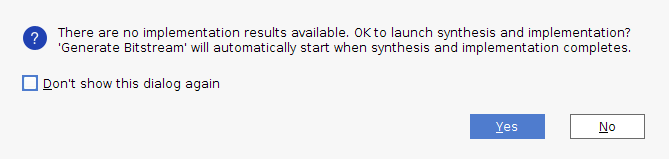
\includegraphics[width=\textwidth]{no_synthesis_results}
    };
    \begin{scope}[x={(image.south east)},y={(image.north west)}]
        \node (start) at (0.93,0.2) {};
        \node [left of=start, xshift=-1.2cm] (end) {};
        \draw [arrow] (start) -- node [midway, black] {} (end);
    \end{scope}
    \end{tikzpicture}
\end{center}

A window like that shown below will pop-up.
The default options are fine, so press OK to continue with generating the bitstream.
You can check "Don't show this dialog again" to always use the default settings.

\begin{center}
    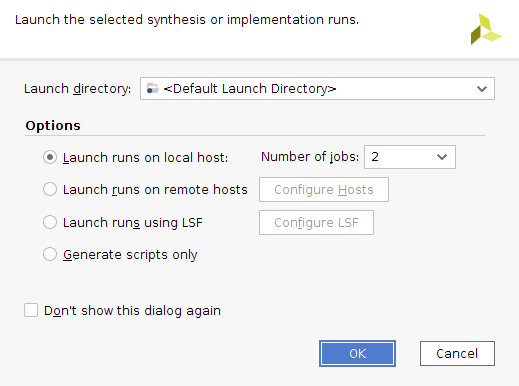
\includegraphics[width=\textwidth]{launch_runs}
\end{center}

If Generate Bitstream completes successfully, then the following window will pop-up.
Selecting an option here is optional, but we want to open the hardware manager next to program
the FPGA so select that option and then OK.

\begin{center}
    \begin{tikzpicture}[arrow/.style={-latex, line width=10pt, darkred!70}]
    \node[anchor=south west,inner sep=0] (image) at (0,0)
    {
        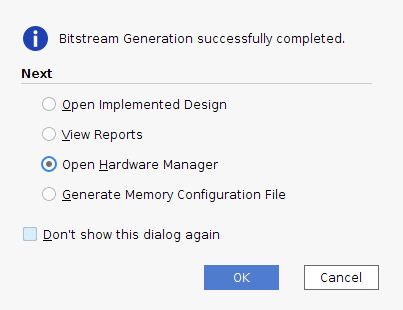
\includegraphics{bitstream_complete}
    };
    \begin{scope}[x={(image.south east)},y={(image.north west)}]
        \node (start) at (0.75,0.47) {};
        \node [left of=start, xshift=-1.2cm] (end) {};
        \draw [arrow] (start) -- node [midway, black] {1} (end);

        \node (start) at (0.603,0.38) {};
        \node [below of=start, yshift=-1.2cm] (end) {};
        \draw [arrow] (start) -- node [midway, black] {2} (end);
    \end{scope}
    \end{tikzpicture}
\end{center}

The hardware manager view will open where you can click on Open target and then Auto Connect.
Everything before this step can be done without the board connected, but now make sure the board
is connected via USB so we can connect to and program the FPGA.

\begin{center}
    \begin{tikzpicture}[arrow/.style={-latex, line width=10pt, darkred!70}]
    \node[anchor=south west,inner sep=0] (image) at (0,0)
    {
        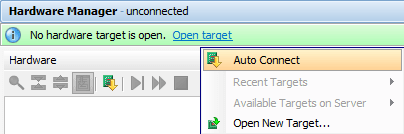
\includegraphics{program_auto_connect}
    };
    \begin{scope}[x={(image.south east)},y={(image.north west)}]
        \node (start) at (0.78,0.74) {};
        \node [left of=start, xshift=-1.2cm] (end) {};
        \draw [arrow] (start) -- node [midway, black] {1} (end);

        \node (start) at (0.95,0.55) {};
        \node [left of=start, xshift=-1.2cm] (end) {};
        \draw [arrow] (start) -- node [midway, black] {2} (end);
    \end{scope}
    \end{tikzpicture}
\end{center}

If the board connected successfully the board and FPGA will show up and the option to Program
device shows up.

\begin{center}
    \begin{tikzpicture}[arrow/.style={-latex, line width=10pt, darkred!70}]
    \node[anchor=south west,inner sep=0] (image) at (0,0)
    {
        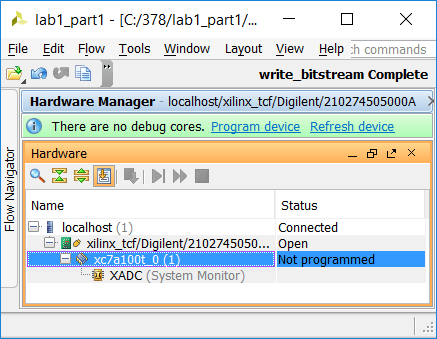
\includegraphics[width=\textwidth]{program_program}
    };
    \begin{scope}[x={(image.south east)},y={(image.north west)}]
        \node (start) at (0.82,0.625) {};
        \node [left of=start, xshift=-1.2cm] (end) {};
        \draw [arrow] (start) -- node [midway, black] {} (end);
    \end{scope}
    \end{tikzpicture}
\end{center}

The .bit file we just generated should be automatically selected, but if not add its path here.
We aren't using debug probes so leave that section blank.
Click Program to program your FPGA.

\begin{center}
    \begin{tikzpicture}[arrow/.style={-latex, line width=10pt, darkred!70}]
    \node[anchor=south west,inner sep=0] (image) at (0,0)
    {
        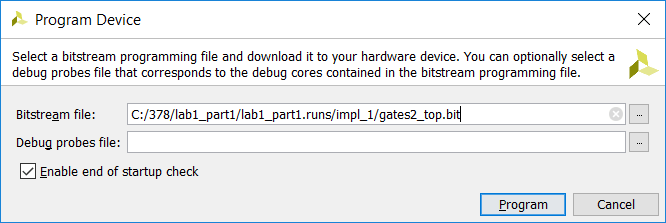
\includegraphics[width=\textwidth]{program_select_file}
    };
    \begin{scope}[x={(image.south east)},y={(image.north west)}]
        \node (start) at (0.965,0.084) {};
        \node [left of=start, xshift=-1.2cm] (end) {};
        \draw [arrow] (start) -- node [midway, black] {} (end);
    \end{scope}
    \end{tikzpicture}
\end{center}

%\section{Programming Flash (OPTIONAL)}
%The FPGA's configuration is volatile, meaning it is lost when it loses power.
%Flash devices on the other hand are non-volatile, so they will keep their stored files even
%without power.
%The Nexys4 board has a flash memory onboard that we can use to store the FPGA configuration file.
%Using this is completely optional for labs, but for the final project presentations you will need
%to have the configuration loaded in flash so that you don't waste time programming the board.
%The first thing we have to do is tell Vivado to generate a bin file during the Generate
%Bitstream step.

% FIGS

%Now re-run Generate Bitstream and connect to the hardware server.

% FIGS

%Add a memory device by right-clicking on the part number and then selecting Add Configuration
%Memory Device...